\documentclass[conference]{IEEEtran}
\IEEEoverridecommandlockouts
% The preceding line is only needed to identify funding in the first footnote. If that is unneeded, please comment it out.
%\usepackage{cite}
\usepackage{amsmath,amssymb,amsfonts}
\usepackage{algorithmic}
\usepackage{graphicx}
\usepackage{textcomp}
\usepackage{xcolor}
\def\BibTeX{{\rm B\kern-.05em{\sc i\kern-.025em b}\kern-.08em
    T\kern-.1667em\lower.7ex\hbox{E}\kern-.125emX}}

% Self-added
\usepackage[style=ieee,dashed=false, urldate=long]{biblatex}
\addbibresource{bibliography.bib}
\usepackage{subcaption}
    
\begin{document}

\title{Sweeping Strategies for an Autonomous Minesweeping Robot\\}

\author{\IEEEauthorblockN{Henrique Rodrigues}
\IEEEauthorblockA{\textit{Informatics Engineering} \\
\textit{Ghent University}\\
Ghent, Belgium \\
Henrique.Rodriques@UGent.be}\\
\IEEEauthorblockN{Lander Verloove}
\IEEEauthorblockA{\textit{Electrical Engineering (CIT)} \\
\textit{Ghent University}\\
Ghent, Belgium \\
Lander.Verloove@UGent.be}

\and

\IEEEauthorblockN{Flor Sanders}
\IEEEauthorblockA{\textit{Electrical Engineering (CIT)} \\
\textit{Ghent University}\\
Ghent, Belgium \\
Flor.Sanders@UGent.be}\\

\IEEEauthorblockN{Lauren Van De Ginste}
\IEEEauthorblockA{\textit{Industrial Systems Engineering (ISyE)} \\
\textit{Ghent University}\\
Kortrijk, Belgium \\
Lauren.VanDeGinste@UGent.be}
}

\maketitle

\begin{abstract}
Landmines still cause harm to a lot of innocent people around the world. Planted mines stay active for years and cannot discriminate between civilians and soldiers. Demining is the only long term solution, but is mostly difficult and costly. To limit accidents during demining, robots can be used for controlled detonation. The rise of autonomous robots could even speed-up the demining process and save thousands of lives. In this paper, autonomous demining is explored by testing and evaluating various demining strategies.
\end{abstract}


\begin{IEEEkeywords}
Robotics, Landmines, ROS, Gazebo, Turtlebot
\end{IEEEkeywords}

\section{Introduction \label{sec:Introduction}}
Even though 164 countries joined the 1997 Mine Ban Convention, more than 60 countries worldwide are still contaminated by landmines \cite{InternationalCampaigntoBanLandmines2016} \cite{InternationalCampaigntoBanLandmines2020}. Landmines are containers of explosive material with detonating systems that are triggered by contact with a person or vehicle. They are designed to incapacitate that person or vehicle through damage caused by an explosive blast, fragments, or, in the case of some antitank mines, a jet of molten metal \cite{Chiovelli2018}. There are two main types of mines: anti-personnel (figure \ref{fig:anti-personnelmine}) and anti-tank mines.

\begin{figure}[htbp]
\centerline{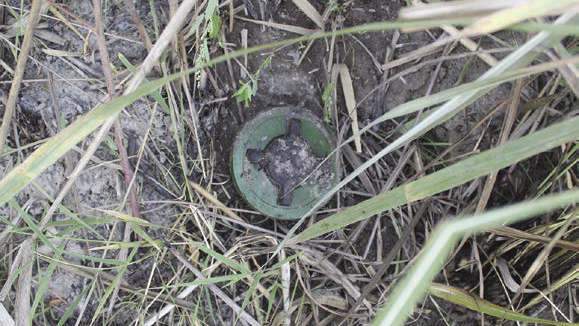
\includegraphics[width=55mm]{PMN-2s.png}}
\caption{A PMN-2 antipersonnel mine (Panj, Tajikistan) \cite{InternationalCampaigntoBanLandmines2020a}}
\label{fig:anti-personnelmine}
\end{figure}

The main problem of landmines is that they, once planted, stay active for years and cannot discriminate between civilians and soldiers \cite{Hiznay2003}. Peace agreements may be signed and hostilities may cease, but landmines and explosive remnants of war (ERW) are an enduring legacy of conflict. In 2019, at least 5,554 casualties of mines were recorded: 2,170 people were killed, 3,357 people were injured, and for 27 casualties the survival status was unknown \cite{InternationalCampaigntoBanLandmines2020}. \\

There are four main pillars that aid in reducing and eliminating the harm mines cause: risk education, clearance, victim assistance and stockpile destruction. The only long term solution is off course banning mines and demining contaminated areas. Demining is more than only disarming or controlled detonation of landmines. It is the set of activities that lead to the removal of mines, including survey, mapping, clearance, marking, and the handover of cleared land \cite{InternationalCampaigntoBanLandmines2020}.
The cost of mine clearance is quite high and frequently exceeds the budget of poor countries that suffer from mines. Next to budget, the mine removal operation is usually performed manually, which is a slow and dangerous process. Therefore, demining robots are on the rise. They have become a viable alternative to perform such dangerous task instead of humans \cite{Jaradat2018}. In literature the importance of autonomous navigation and good controllabity is highlighted \cite{Jaradat2018}. The robot should be able to deal with connection problems and make planning decision on it's own. This is seen as a crucial step in improving efficiency of search and cleaning \cite{Dogru2019}. In this paper different autonomous mine sweeping strategies are discussed. Section \ref{sec:Approach} describes the implemented strategies and related simulations and section \ref{sec:Results} compares the results of the different mine sweeping strategies. Section \ref{sec:Challenges} highlights the challenges. This paper ends with a conclusion and outlook towards future research (section \ref{sec:Conclusion}).


\section{Approach \label{sec:Approach}}

The strategies discussed in this paper are all tested in simulation. Therefore the approach is twofold. First there is the implementation of a simulated environment for testing. Second there is the implementation of algorithms for mine sweeping intended to be pluggable into a real robot. \\

The algorithms and simulations are based on and developed for the Turtlebot 3 Burger model. This robot does not have the physical properties required for demining, but it is a perfect robot for development purposes. Simulation files are available and the most important sensors for autonomous driving are present, mainly the LIDAR. Figure \ref{fig:TurtlebotComponents} shows the main components of the robot. Some specifications are highlighted in table \ref{tab:TurtlebotSpecs}. The Turtlebot is programmed via the Robot Operating System (ROS) and simulated via Gazebo. ROS is a set of software libraries and tools that help building robot applications and Gazebo on the other hand offers the ability to accurately and efficiently simulate robots in complex indoor and outdoor environments \cite{OpenSourceRoboticsFoundation2020} \cite{OpenRobotics2020}.


\begin{table}[htbp]
\caption{Turtlebot 3 Burger: specifications \cite{Robotis2020}}
\begin{center}
\begin{tabular}{|c|c|}
\hline
\textbf{Item}&\textbf{Burger} \\
\hline
Maximum Translational Velocity & 0.22 m/s\\ \hline
Maximum Rotational Velocity & 2.84 rad/s\\ \hline
Maximum Payload & 15 kg\\ \hline
Size (L x W x H) & 138 mm x 178 mm x 192 mm \\ \hline
Operating Time & 2h30 \\ \hline
Sensors & HLS-LFCD2\\ 
& 3-axis gyroscope\\ 
& 3-axis accelerometer\\ 
& 3-axis magnetometer\\ 
\hline
\end{tabular}
\label{tab:TurtlebotSpecs}
\end{center}
\end{table}

\begin{figure}[htbp]
\centerline{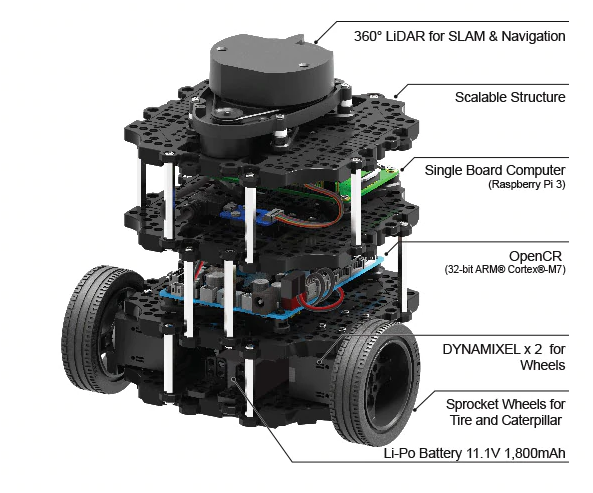
\includegraphics[width=55mm]{TB_Components.png}}
\caption{Turtlebot 3 Burger: most important components \cite{Robotis2020}}
\label{fig:TurtlebotComponents}
\end{figure}

\subsection{Simulation}
To test different algorithms in simulation, testing environments of different sizes and difficulty levels are created using the simulation description format (SDF) for world creation in Gazebo. Obstacles are placed within a walled area. Hills and rough terrain are disregarded. The obstacles are adopted and resized from the standard Gazebo models library \cite{GazeboModels2020}. The robot itself is spawned into the world and can only work within the walled area. The mines are invisible to the robot and are 20\% the size of the Turtlebot in cross section. They are randomly distributed into the area and simulated by red dots. When driving over them (and thus detonating them) they change color to green. This way it is easy to keep track of the demining during live simulation, it also indicates how the selected strategy is doing.\\

To detect a collision between the robot and a mine in simulation, they are both assumed to be disks in a plane with a radius of 10.5 cm and $\frac{10.5}{\sqrt{5}}$ cm respectively. Once the disks of the mine and robot have overlap, the mine is ‘detonated’ and replaced with a green one. Those actions do not affect the robot in any way. However, the number of cleared mines is published to a topic to which the robot can subscribe and detect the event of a detonation. \\


Figure \ref{fig:GazeboEnvironment} shows the three simulated worlds. The worlds differ in size, shape and number of obstacles. Next to describing the world and its obstacles, the SDF files determine the number of mines and simulation parameters (e.g. number of solver iterations, real time update rate etc.) for optimal simulation. During simulation all required data is logged to text files. The original distribution of mines, detonation time and robot position are logged. Simulations can be started with a custom script where duration, number of simulations, strategy and environment can be set. To visually assess a simulation, a figure is created which shows the path and sequence of detonation (Figure \ref{fig:SingleRunTraject} under section \ref{sec:Results}).


\begin{figure}[htbp]
    \centering
        \begin{subfigure}[b]{70mm}
            \centering
            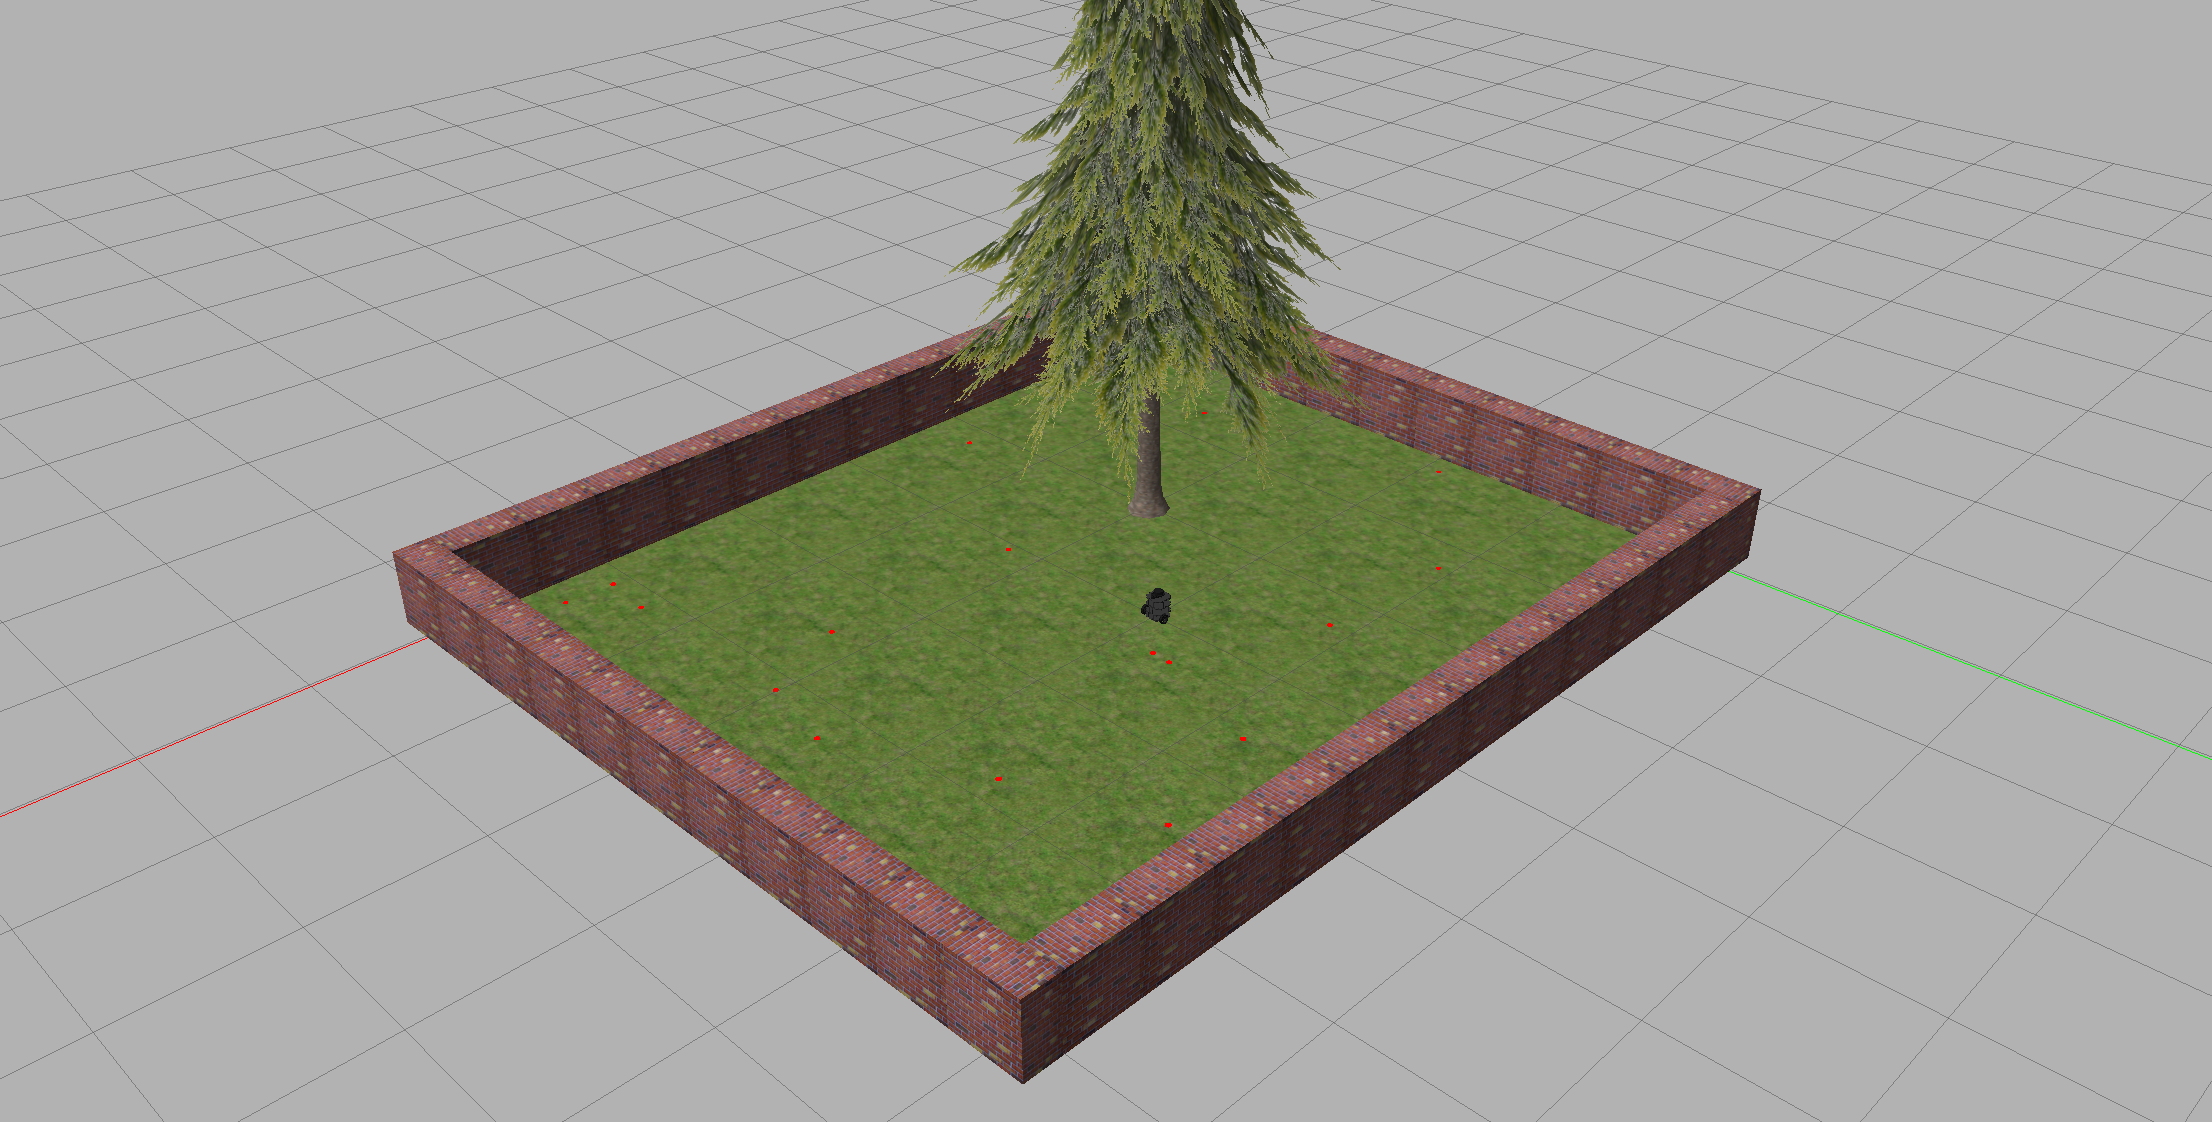
\includegraphics[width=75mm]{W1.png}
            \caption{Small (30 m²)}
            \label{Gazebo-small}
        \end{subfigure}
        \begin{subfigure}[b]{70mm}
            \centering
            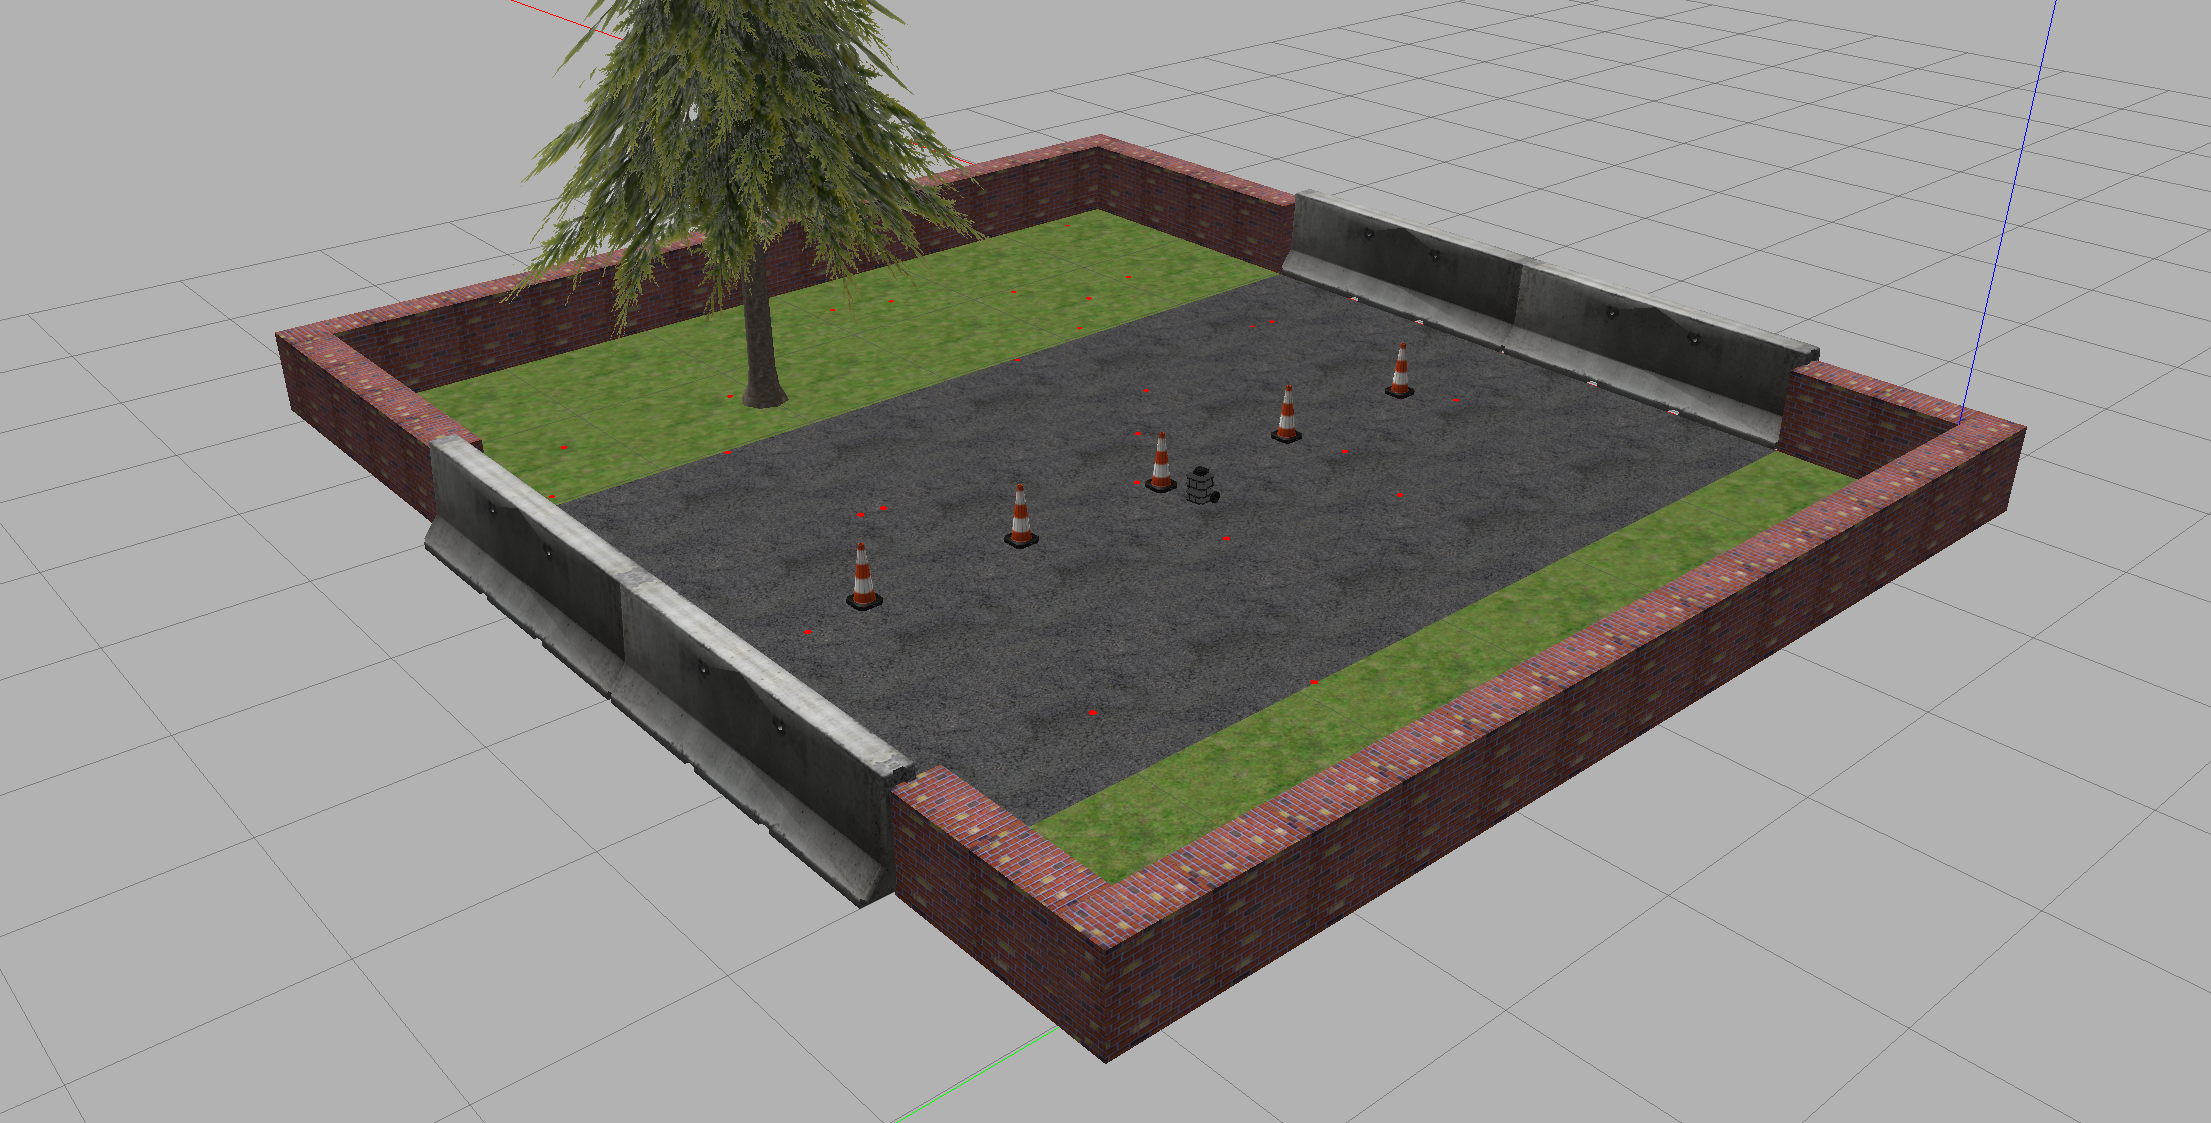
\includegraphics[width=75mm]{W2.png}
            \caption{Medium (42 m²)}
            \label{Gazebo-medium}
        \end{subfigure}
        \begin{subfigure}[b]{70mm}
            \centering
            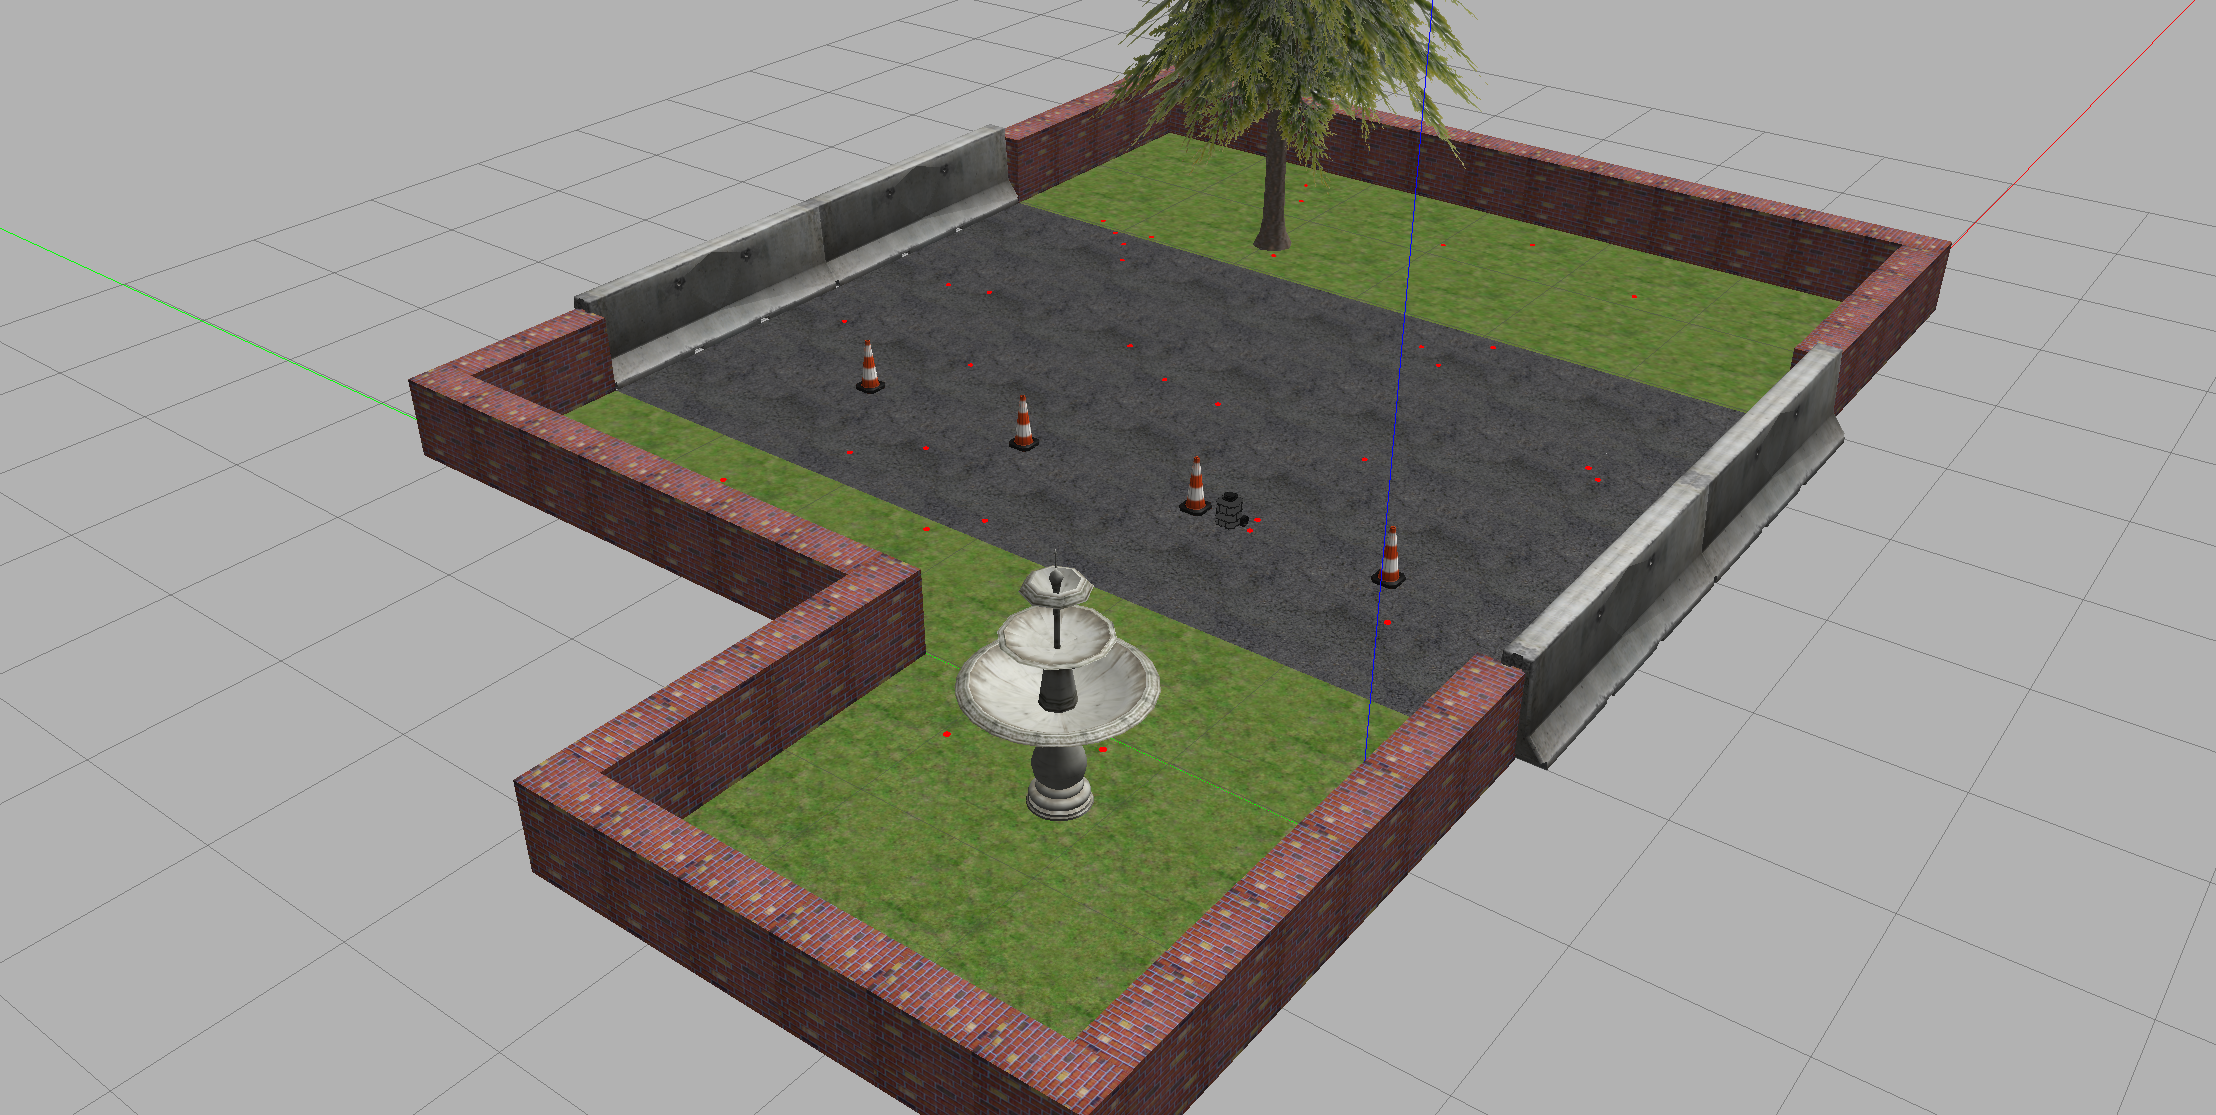
\includegraphics[width=75mm]{W3.png}
            \caption{Large (47 m²)}
            \label{Gazebo-large}
        \end{subfigure}
    \caption{Test environments in Gazebo}
    \label{fig:GazeboEnvironment}
\end{figure}


\subsection{Sweeping Strategies}

We distinguish two types of sweeping strategies for sweeping an area and detonating mines: basic and smart strategies. The basic, mostly 'dumb', strategies attempt to drive around in a predefined pattern, only using the available data from the sensors to avoid crashing into obstacles. They thus do not plan ahead. The smart strategies on the other hand involve mapping the environment as the robot moves so that a reference to the robot position can be obtained and the optimal sweeping strategy defined. These two types of sweeping strategies are also implemented in current robot vacuum cleaners \cite{Casas2006}.\\

To have a good baseline for comparing different sweeping strategies it all starts with a totally random sweeping of the area. The principle of this first basic strategy is as seen in figure \ref{fig:Dumb-RandomRoomba}. The robot just drives forward, until an obstacle is detected and then turns randomly. Because we work inside a walled area it can be expected that this random algorithm works quite well and has a high chance of detonating all mines if the robot drives around long enough. Next, it is explored if making basic strategies smarter, results in better and faster sweeping. Is an autonomous planning robot required? What if the robot follows a path (without knowing the map) while avoiding obstacles? In figure \ref{fig:Dumb_SquareSpiral} and \ref{fig:Dumb_Worm} the theoretical paths of two extra basic algorithms are shown. Note that no obstacles are present in the figures. 

\begin{figure}[htbp]
     \centering
     \begin{subfigure}[b]{27mm}
         \centering
         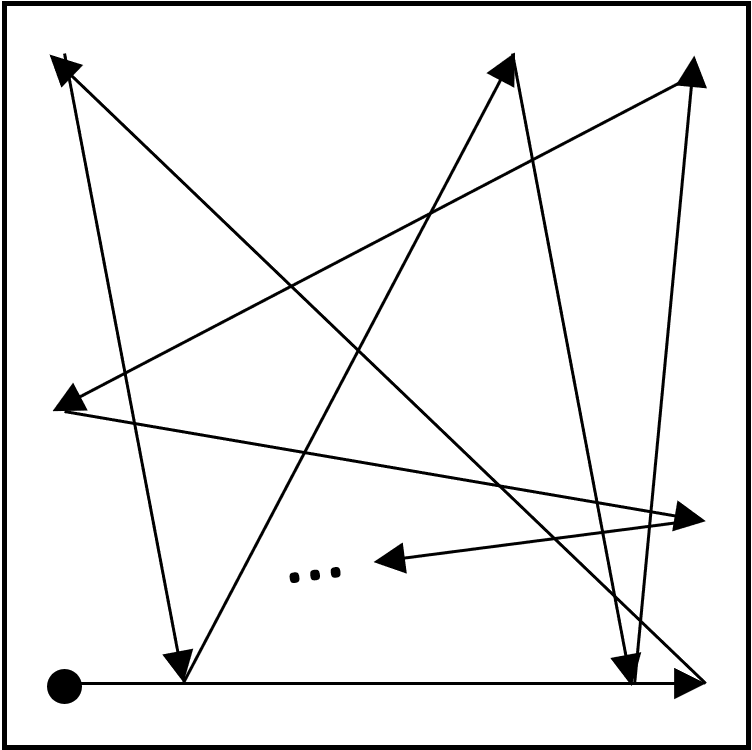
\includegraphics[width=18mm]{Dumb_RandomRoomba.png}
         \caption{Random Roomba}
         \label{fig:Dumb-RandomRoomba}
     \end{subfigure}
     \begin{subfigure}[b]{27mm}
         \centering
         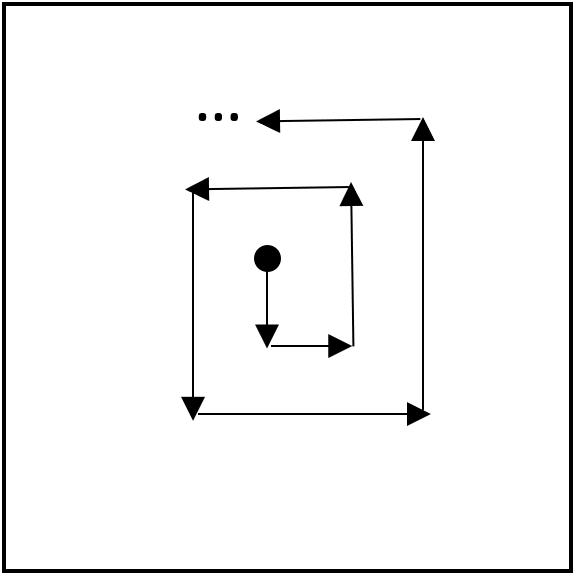
\includegraphics[width=18mm]{Dumb_SquareSpiral.png}
         \caption{Square Spiral}
         \label{fig:Dumb_SquareSpiral}
     \end{subfigure}
     \begin{subfigure}[b]{27mm}
         \centering
         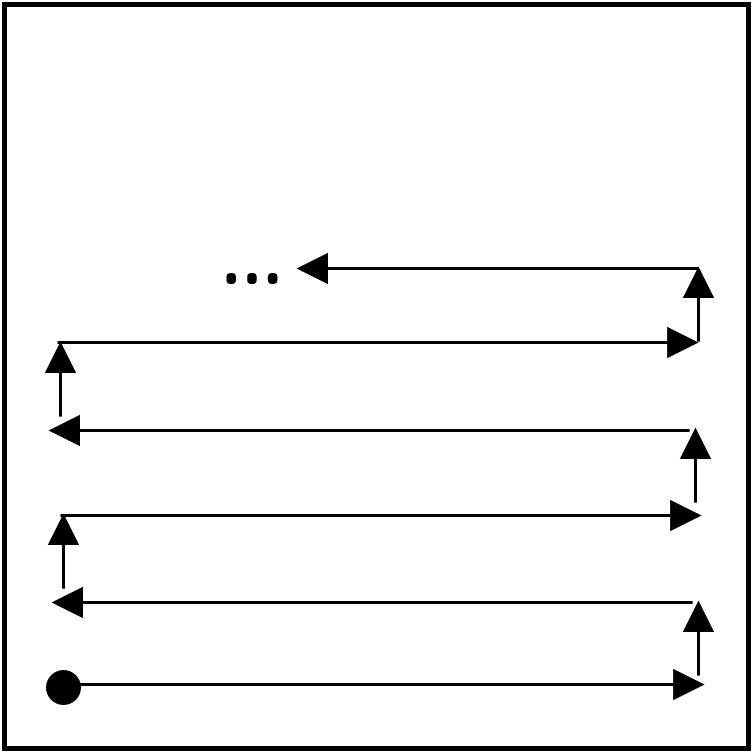
\includegraphics[width=18mm]{Dumb_Worm.png}
         \caption{Worm}
         \label{fig:Dumb_Worm}
     \end{subfigure}
        \caption{Three basic sweeping strategies}
        \label{fig:three graphs}
\end{figure}

Even without running a simulation it is understandable that the square spiral and worm algorithm will not work that well. In an area without obstacles, it could run quite satisfyingly but drift would result in deviations from the desirable path. Also when obstacles are present the robot will have to re-position without knowing where he is. Therefore the expectations are quite low.\\

To have more efficient and planned sweeping, it is important that the robot knows where it is and that it can handle the environment well. In fact learning maps under pose uncertainty is often referred to as the simultaneous localization and mapping (SLAM) problem \cite{Grisetti2010}. To have an idea where the robot is, it could use GPS while it works in an outdoor environment, however with only GPS it cannot know where obstacles are. For this reason we opted for a SLAM-based approach using the LiDAR sensor. Based on mapping and planning simultaneously, three smart algorithms are implemented. These smart algorithms are developed as to extract as much information from the available sensor data as possible. They make use of the gmapping SLAM algorithm, which combines the robot's odometry and the measurements of the Laser Distance Sensor (LDS) to build a map of its environment \cite{gmapping}. Additional to the map and its pose within it, the robot keeps track of the places it has visited as well. Since the robot only sporadically receives updates about the map, a linear interpolation with ten points is performed between its previous and current positions. All of the above is visualized in figure \ref{fig:slambotinfo}.\\

\begin{figure}[htbp]
\centerline{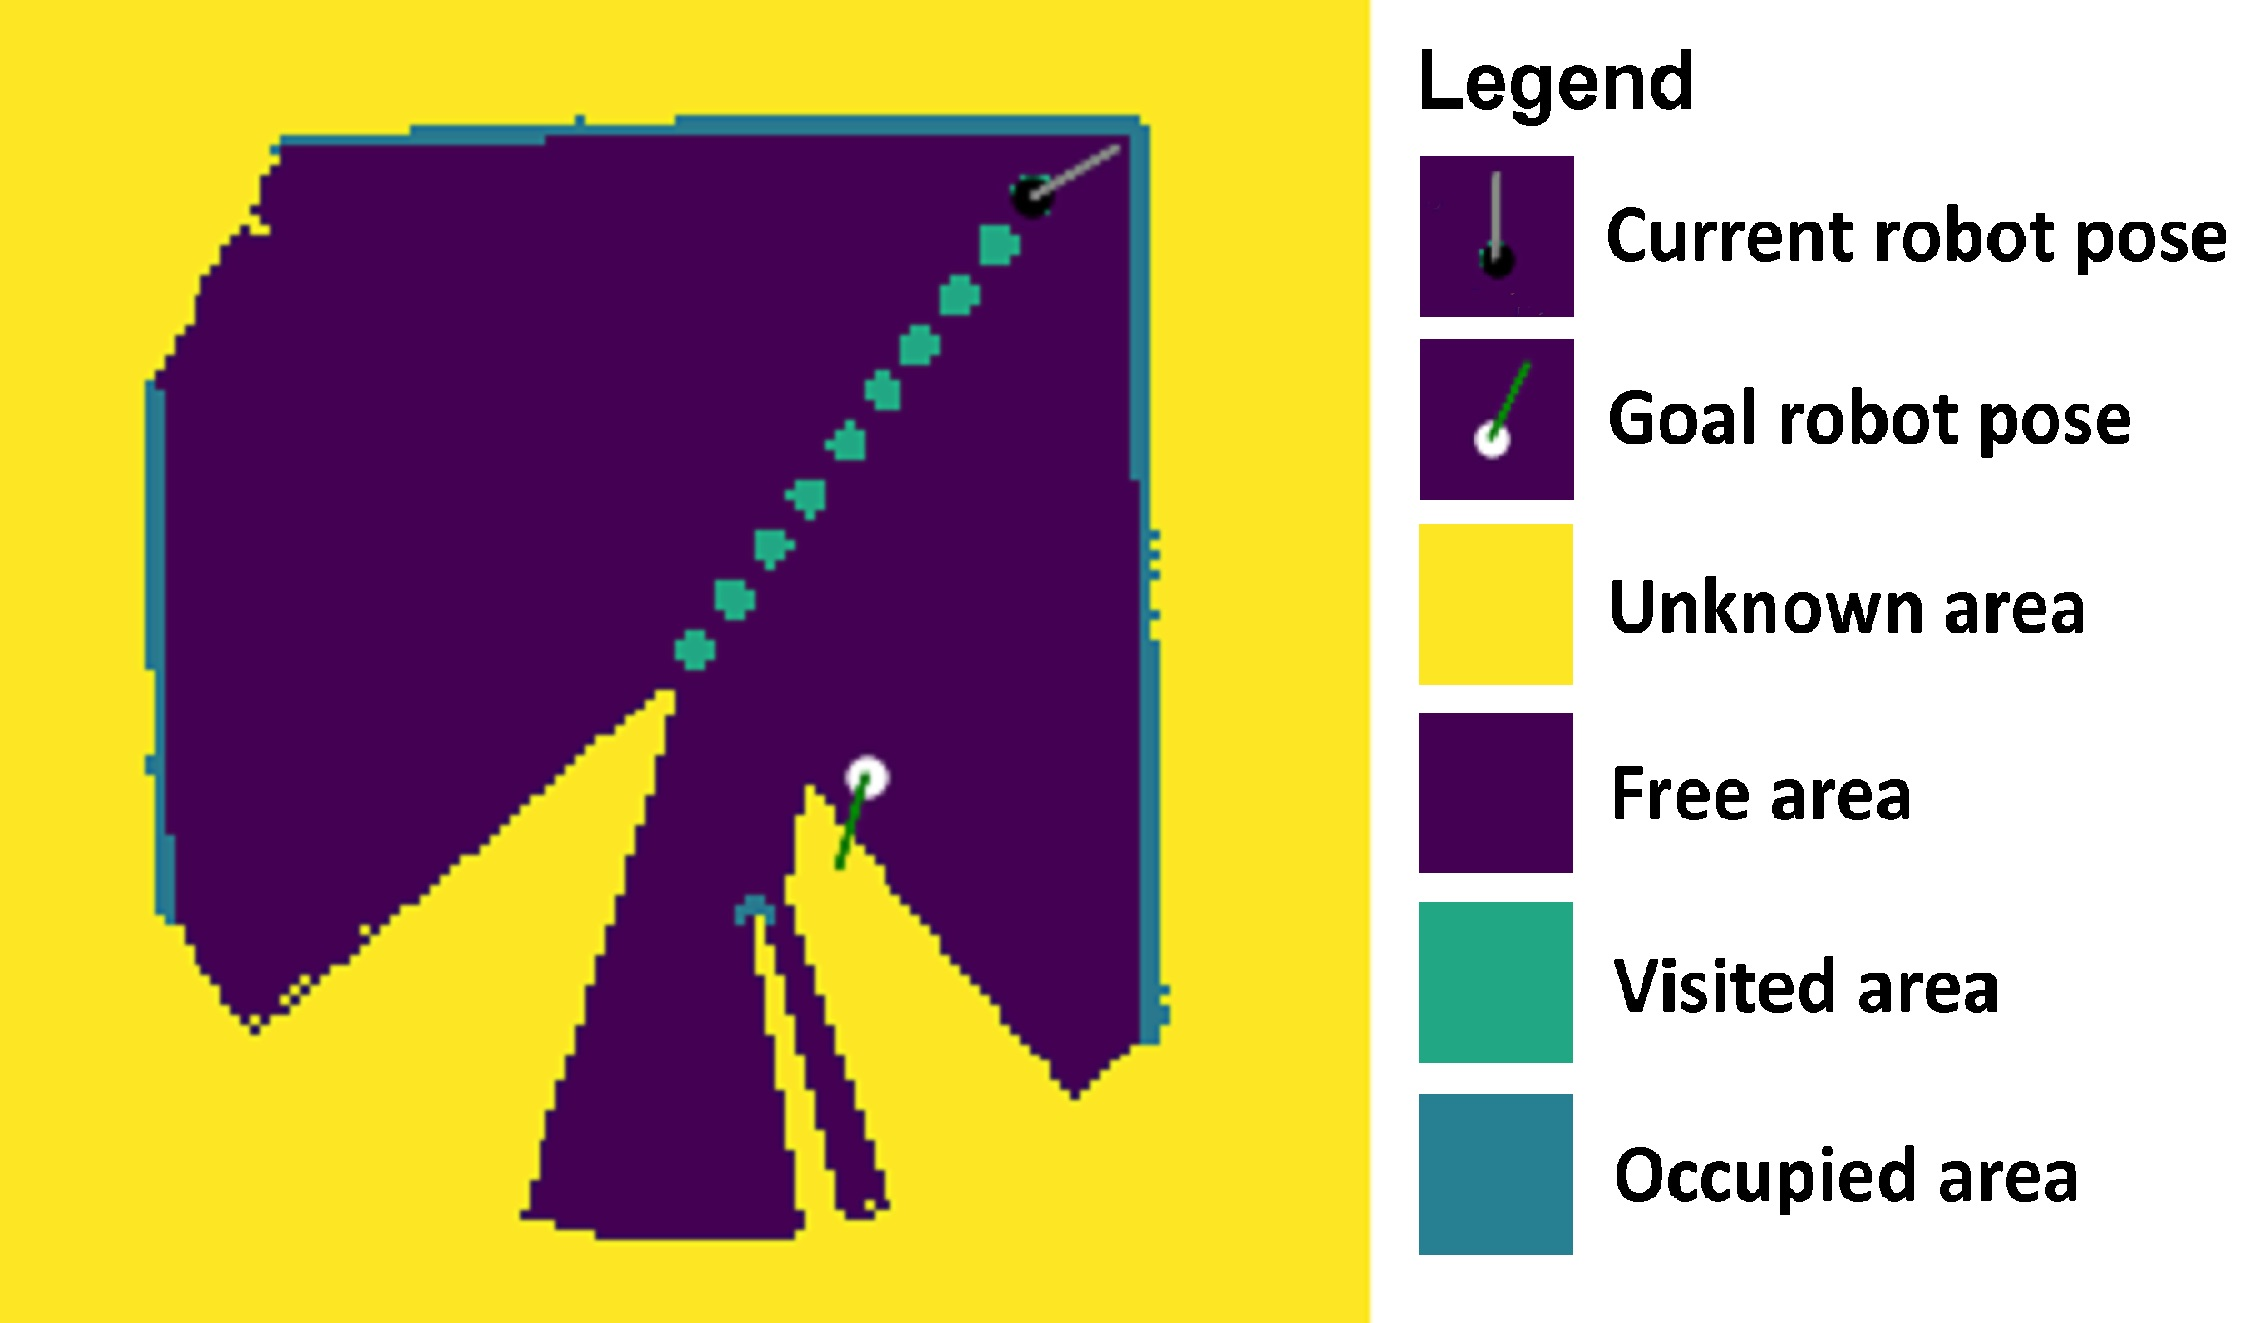
\includegraphics[width=63mm]{SLAM_Info.jpg}}
\caption{Information the robot keeps track of.}
\label{fig:slambotinfo}
\end{figure}

Rather than driving in a predetermined pattern as with the basic strategies, another approach is here taken. As in the simulations the mine positions are random and uncorrelated, no assumptions can be made about where they will be. The ideal scenario is then to have the robot visit every spot on the map as quickly as possible. To achieve this we use the information described in the previous paragraph to choose a new goal from the unvisited places that are at least 12.5 cm away from any occupied area. The choice is made in a random fashion according to a probability distribution. Here we make a distinction between three different strategies:
\begin{enumerate}
    \item Smart - Random: Makes use of a uniform probability distribution. Each of the available options has equal probability to be selected.
    \item Smart - Far: The probability for a position to be selected is proportional to the distance squared. A bias towards positions that are further away is introduced, which promotes exploration of new area above sweeping in its direct environment.
    \item Smart - Near: The probability for a position to be selected is inversely proportional to the distance squared. A bias towards samples that are closer by is introduced, which promotes thoroughly sweeping in the robot's direct vicinity before going somewhere else.
\end{enumerate}
After the position for the goal is selected, the orientation is chosen in such a way that only minimal corrections are required upon arrival. In order to reach our selected goal we make use of the ROS navigation stack, with the most important package being move\_base. As described in \cite{move_base} this package combines a global and a local planner, each building their own cost map, to determine the optimal path to the goal. The above steps are repeated until all reachable places have been visited. The main challenges are in optimally covering the area and detonating mines as quickly as possible.

\section{Results \label{sec:Results}}

Because of the stochastic character of simulations, multiple runs, with the same settings, per world and strategy are needed to assess the performance in a reproducible way. Table \ref{tab:SimSet} displays the settings used for all simulations. The number of mines and time are proportional to the area. That way they each have the same mine density and same time per square meter to sweep the area. The main difference in performance that can be expected between worlds should be due to the number of obstacles or shape of the terrain. The mines are always randomly distributed within the complete walled area at start-up of the simulation.

\begin{table}[htbp]
\caption{Information on settings for simulations}
\begin{center}
\begin{tabular}{|c|c|c|c|}
\hline
\textbf{Item}&\multicolumn{3}{|c|}{\textbf{Gazebo Test Environment}} \\
\cline{2-4} 
&\textbf{Small}&\textbf{Medium}&\textbf{Large} \\
\hline
Area [m²] & 30 & 42 & 47 (42 + 5)\\ \hline
Number of mines [\#] & 30 & 42 & 47\\ \hline
Number of obstacle [\#] & 1 & 6 & 6\\ \hline
Duration of simulation [sec.] & 1800 & 2520 & 2820\\ \hline
Starting position [(x;y)] & (0.5; 0.5) & (0.5; 0.5) & (0.5; 0.5)\\ \hline
\end{tabular}
\label{tab:SimSet}
\end{center}
\end{table}

\begin{table}[htbp]
\caption{Number of simulations}
\begin{center}
\begin{tabular}{|c|c|c|c|}
\hline
\textbf{ Strategy} &\multicolumn{3}{|c|}{\textbf{Gazebo Test Environment}} \\
\cline{2-4} 
 & \textbf{Small} & \textbf{Medium} & \textbf{Large} \\
\hline
Random Roomba (B) & 30 & 30 & 4 \\
\hline
Square Spiral (B) & 15 & 15 & 4 \\
\hline
Worm (B) & 15 & 15 & 4 \\
\hline
Smart Random (S) & 15 & 15 & 4\\
\hline
Smart Near (S) & 15 & 10 & 4 \\
\hline
Smart Far (S) & 15 & 10 & 4 \\
\hline

\multicolumn{4}{l}{(B) Basic sweeping strategy; (S) Smart sweeping strategy}\\
\end{tabular}
\label{tab:SimRuns}
\end{center}
\end{table}

When looking into the results of a single run a first idea about the performance of the strategy can be gathered. Figure \ref{fig:SingleRunTraject} shows the traject with the mine distributions of two simulation runs. We can see in this single runs that the smart algorithm plans it's trajectory around obstacles, while the random strategy just stops before an object. Tweaking the penalty for getting close to object is important to be sure no mines are missed. The smart-far algorithm here displayed seems to stay away a bit too far from objects, resulting in less mines close to objects cleared on the long run. The observations here mentioned should be reflected in the analysis further on.\\

\begin{figure}[htbp]
     \centering
     \begin{subfigure}[b]{70mm}
         \centering
         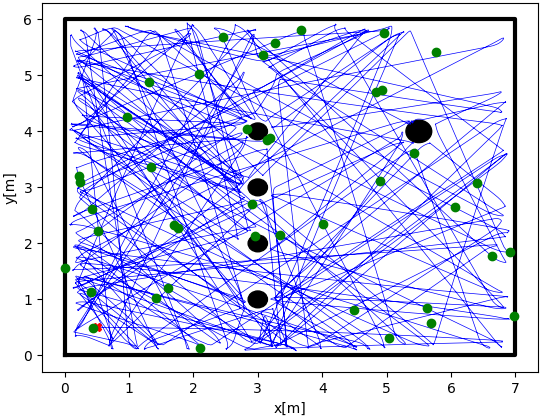
\includegraphics[width=67mm]{Traject_Medium_RandomRoomba_10-12-2020_140644_Mines.png}
         \caption{Random Roomba (Basic strategy)}
         \label{fig:RandomRoombaSingleRun}
     \end{subfigure}
     \begin{subfigure}[b]{70mm}
         \centering
         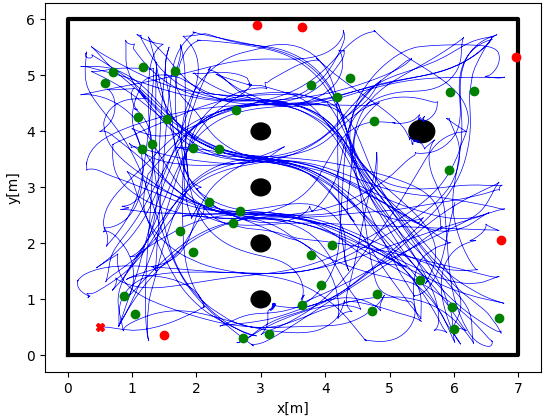
\includegraphics[width=67mm]{Traject_Medium_SmartFar_11-12-2020_215635_Mines.png}
         \caption{Smart Far (Smart strategy)}
         \label{fig:SlamXSingleRun}
     \end{subfigure}
        \caption{Single run robot trajectory of sweeping in medium environment}
        \label{fig:SingleRunTraject}
\end{figure}

As said before, because the simulations are stochastic and performance can thus variate, no real conclusions can be drawn from single runs. Therefore some key performance indicators (KPI) are defined based on multiple simulations. Table \ref{tab:SimRuns} shows the number of intended runs per environment. The main analysis is based around the small and medium environment. As the number of runs for the large environment were quite low due to time restrictions, we were unable to draw any new and statistically significant conclusions from this data. To note, on an average pc, one simulation takes approximately one and a half hour to simulate 47 minutes. Nevertheless as the number of obstacles and mine density is the same as in the medium environment, not a big difference in results is expected between the medium and large world. \\

The first KPI identifies how good the algorithms are at finding mines in the early stages of their operation. The time until 40\% of the distributed mines are detonated, is calculated based on all runs per strategy per world. Figure \ref{fig:BP40} gives a box plot visualization for this KPI for the strategies in the small and medium environments. Inspecting these thoroughly, the following conclusions are drawn. First, it can be seen that the random roomba algorithm, with an average time of 549.40 seconds till 40\% of mines are cleared in the small world and 463.72 seconds in the medium world, scores very well in general, which could be expected when seeing its driving pattern in figure \ref{fig:RandomRoombaSingleRun}. Thanks to the ideal environment, the robot is able to cover most of the area by simply driving around randomly. The performance of the smart algorithms is a bit of a mixed bag. For example the smart far algorithm has an average time of 592.26 seconds in the small world and 941.93 seconds in the medium world till it cleares 40\% of the mines. To understand why, we need to take a good look at how the algorithms work. The main reason the smart algorithms don't tend to outperform the random roomba is because the navigation stack avoids getting too close to obstacles or walls, missing the opportunity to clear mines near them. The difference in performance between the variations of the smart algorithms is entirely due to the distance bias in their choice of goal. The smart near algorithm is penalized for two reasons. Since it tends to explore less new area it finds less new mines in the short term, which is precisely what this KPI focuses on. Additionally, the robot slows down when nearing its goal as to not overshoot it, which results in a lower average speed for this algorithm. We see then that exploratory strategies are more suited according to this KPI, which is also confirmed by the good performance of the smart far algorithm in the small world. In the medium environment the performance of the smart far and the smart random is more comparable. This is quite understandable as, since there is often times more area far away from the robot than in its direct vicinity, the smart random algorithm also has an unintended bias towards choosing goals that are far away. The slightly worse median and mean performance for the smart far algorithm can mainly be ascribed to some outliers where it lost time crashing into obstacles with a larger base than top, which the LDS is unable to detect. Unsurprisingly, the worm and square spiral algorithms don't perform all that good. The square spiral strategy doesn't even detonate 40\% of the mines within the simulation time. This can simply be explained by their difficulty with handling obstacles, which hinder them in their goal to drive in a predefined pattern. The fact that we start driving near a wall does not help in this matter, as this means the robot will encounter obstacles rather quickly.\\

\begin{figure}[htbp]
     \centering
     \begin{subfigure}[b]{85mm}
         \centering
         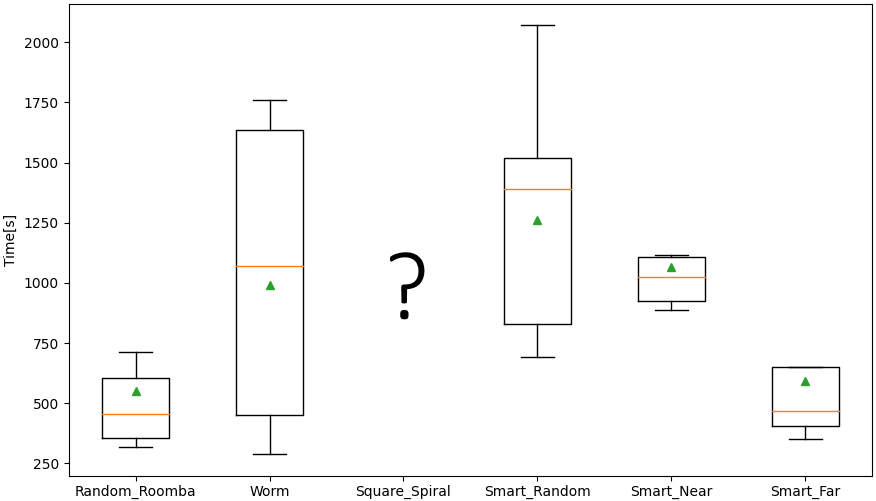
\includegraphics[width=79mm]{Analysis_Small_TimeTill40.png}
         \caption{Small Environment}
         \label{fig:BP40_Small}
     \end{subfigure}
     \begin{subfigure}[b]{85mm}
         \centering
         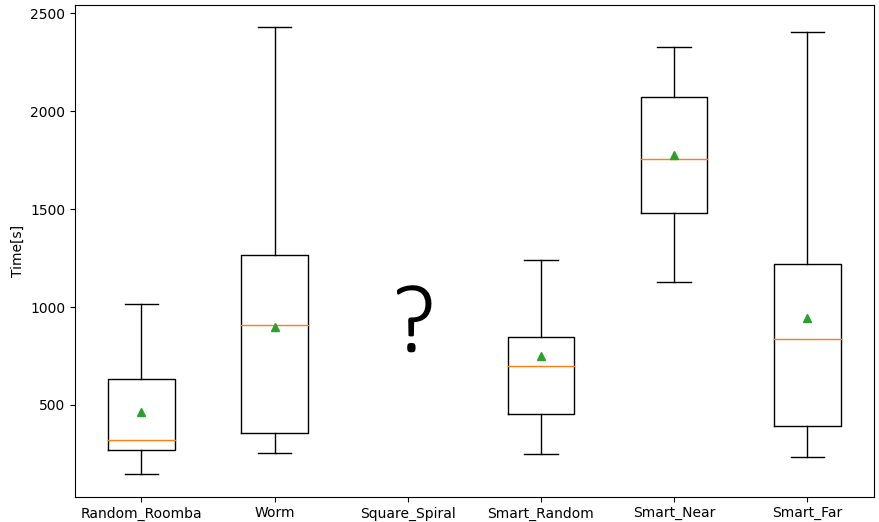
\includegraphics[width=79mm]{Analysis_Medium_TimeTill40.png}
         \caption{Medium Environment}
         \label{fig:BP40_Medium}
     \end{subfigure}
        \caption{Box plots of time till 40\% of mines are detonated}
        \label{fig:BP40}
\end{figure}

The second KPI evaluates the performance of the algorithm over the whole duration of the run, making use of the inter mine detonation time (IMDT) as a performance metric. Figure \ref{fig:BPMin} gives box plots for the second KPI for the strategies in the small and medium environments. We see that when given enough time, most of our algorithms actually perform quite similarly, with smart near falling a bit behind and square spiral being the worst performer of all. As before, random roomba (small: 44.33 seconds, medium: 50.98 seconds) comes out on top, because it covers a lot of area quickly and it also clears more of the mines near obstacles. Of the smart algorithms, the smart far (small: 62.95 seconds, medium: 68.53 seconds) one is the best performer, showing us again that exploratory strategies perform better because they cover more area. We also notice no significant difference between the performance in the small and medium worlds for all algorithms except square spiral. All things being equal, we can conclude that the number of obstacles in the environment has only a marginal influence on the IMDT.\\

So far the overall mine clearance has not been explicitly assessed. An obvious KPI to measure this is the time until all mines are detonated. For our simulations, a fixed simulation time was used. In most cases, this time was not long enough to detonate all mines. Hence, to get a rough estimate the best performing smart algorithm (smart far) and the random roomba algorithm were selected. Thereafter, the average time for every nth mine to be detonated over all simulations in the medium world was calculated, for each of the two strategies. The result is shown in figure \ref{fig:ATUD}. Next, exponential regression was used to fit an exponential curve to this data. Using this curve, the data can be extrapolated to find the simulation time until the last mine is found. With the method described above, 3960 seconds and 2029 seconds are needed to find all the mines for the smart far and random roomba strategy respectively.\\

\begin{figure}[htbp]
    \centering
    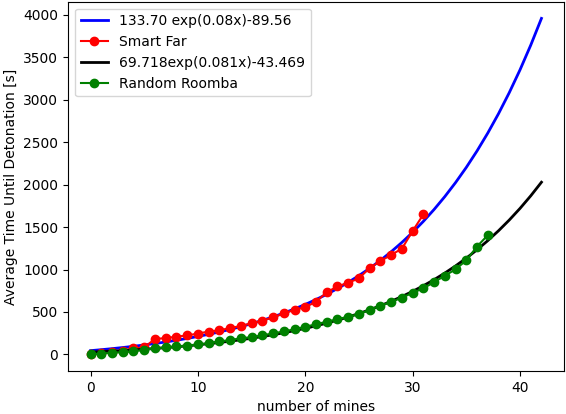
\includegraphics[width=70mm]{Analysis_Medium_AverageTimeUntilDetonation.png}
    \caption{Average time until detonation for smart far and random roomba in the medium world}
    \label{fig:ATUD}
\end{figure}

In hindsight, we do note that the environments seem to be well suited to algorithms such as the random roomba, as it is able to power its way through by simply covering as much area as possible. For areas with a more complex shape, e.g. two rooms separated by a narrow corridor, a larger difference in performance is expected with the smart algorithms coming out on top, since they have the ability to navigate in complex environments.\\

\begin{figure}[htbp]
     \centering
     \begin{subfigure}[b]{85mm}
         \centering
         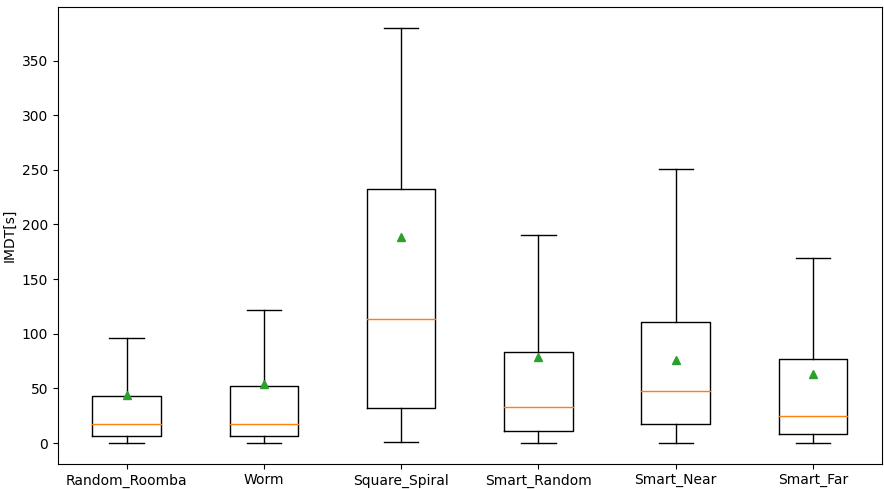
\includegraphics[width=79mm]{Analysis_Small_InterMineDetonationTime.png}
         \caption{Small Environment}
         \label{fig:BPMin_Small}
     \end{subfigure}
    
     \begin{subfigure}[b]{85mm}
         \centering
         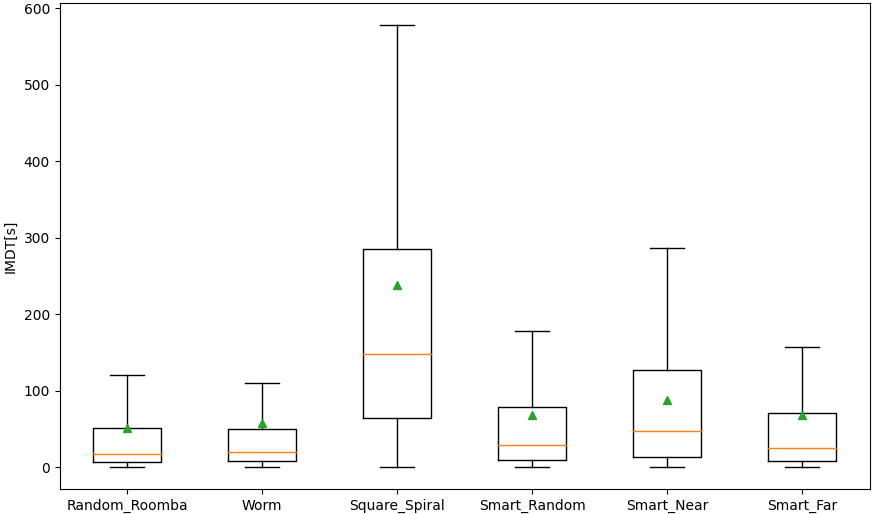
\includegraphics[width=79mm]{Analysis_Medium_InterMineDetonationTime.png}
         \caption{Medium Environment}
         \label{fig:BPMin_Medium}
     \end{subfigure}
        \caption{Box plots of inter mine detonation time (IMDT)}
        \label{fig:BPMin}
\end{figure}

\section{Challenges \label{sec:Challenges}}

Next to the implementation of autonomous mine sweeping in this project being twofold, the challenges are even threefold.\\

Simulation and algorithmic challenges are linked. First, when using simulations for evaluating strategies, a lot of assumptions are made, both intentionally and unintentionally. It's common knowledge that simulating and replicating the exact real world environment is difficult, the so called simulation-to-reality gap is always present. Some simplifications are however intentional. For example, the environments used are completely flat. Hills and rough terrain are disregarded. This is because when driving over rough terrain the LiDAR will start to shake and sensor readings will be less stable. The main problem is that the SLAM problem increases from 3 degrees of freedom to 6. VisualSLAM using RGB camera's could help but has also its drawbacks: influence of sunlight, high data load etc. \cite{Daems2020}. Most objects in the environment are quite simple, however some problems could arise if objects become more complex as well. For example if an object is not tall enough, the sensor doesn't notice it and will bump into it. A different placement of sensors or adding additional sensors is thus advisable. Concluding, when applying the algorithms described in this paper to the real world, some additional difficulties will have to be overcome because of the simulation-to-reality gap. \\

Also in the implementation of the sweeping algorithms themselves a lot of challenges can be identified. Ideally, the values of parameters such as sensor poll rate, object detection threshold, angular and linear speed should be adapted to fit the environment. Then there is the challenge of optimally planning a route in an incomplete map, while avoiding obstacles but not so much as to miss mines in their vicinity. Furthermore, when adding more sensors such as GPS, sensor fusion techniques should be implemented to achieve more precise and reliable data. With all of this however, the limitations on computational resources (largely because of budget) need to be taken into account.\\

A third challenge, which is out of scope of this paper, is the robot hardware. For research purposes, we made use of the Turtlebot platform. However, since this robot is made entirely out of plastic, it is thus not capable of withstanding an explosion: a notable factor when bringing the algorithms to reality. Next to developing algorithms for demining, a lot of research thus remains in constructing the right robot which can withstand the impact, is not disoriented after an explosion and has enough autonomy to completely sweep an area.

\section{Conclusion and Outlook \label{sec:Conclusion}}
Autonomous robots have a lot of potential and can save thousands of lives in the field of demining. They are able to autonomously demine complete areas infected by landmines and thereby reduce the risk while also reducing cost. In this paper six mine sweeping strategies are compared in a virtual environment. They are evaluated using different KPI's and in different situations, concluding after multiple runs that driving around randomly is a good option if enough time is taken into account. However smart strategies, which keep track of where they have been, have the potential to outperform the random strategy and provide more certainty towards total mine clearance. In future research, the algorithms themselves can be improved for flat terrain to cope better with obstacles. However they should also be adopted for rough terrain and other environmental factors. The design of a robot which can withstand explosions should also not be neglected since it can influence sensor position and thus algorithms. The robot here used is made out of plastic and thus only usable for development purposes. By combining the robot design and the development of the sweeping patterns the robot will be able to withstand real world environments. 

\section*{Acknowledgment}

This paper is created in the context of a project assignment for the Robotics course (E019370) taught by prof. Tony Belpaeme and prof. Alain Sarlette a Ghent university during the academic year 2020-2021. The source code is released under an AGPL-3.0 license and can be found at: https://github.ugent.be/robotics-2021/Group-8.


\printbibliography
\vspace{12pt}

\end{document}
